
\section{LBNF/DUNE Project}
\begin{figure}
\caption{LBNF/DUNE overall scheme. The neutrino flux will be produced using existing proton accelerator at Fermilab. Then neutrinos will be registered by the ND, travel 1300 km to the SURF in South Dakota and be registered by the FD. Source of figure: \cite{ref_LBNFweb} }
\label{fig:LBNF_overallScheme}
\centering
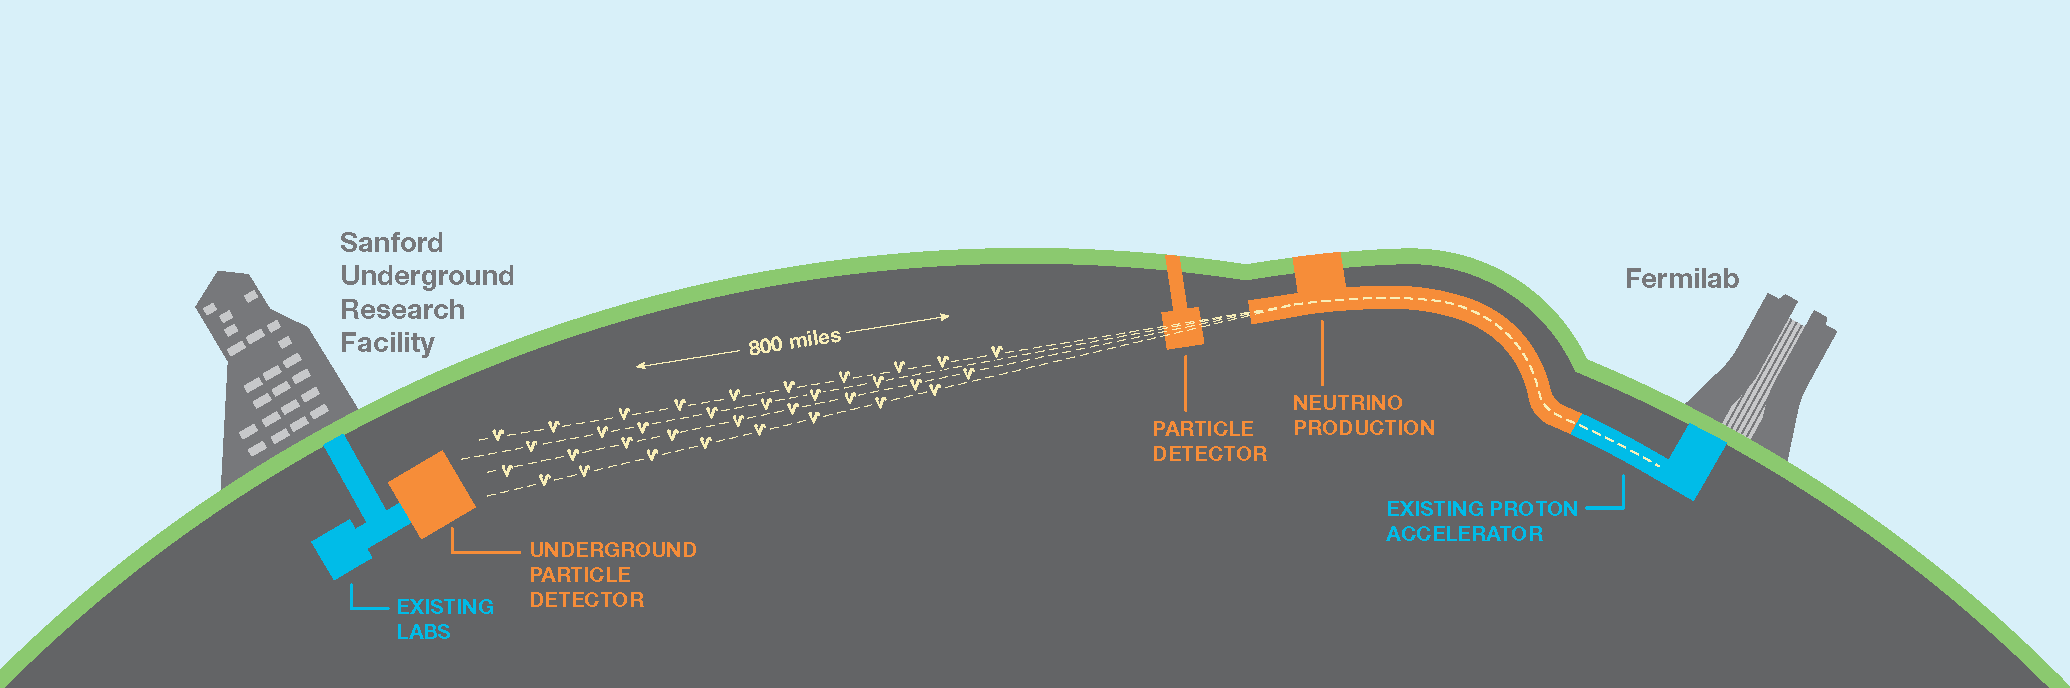
\includegraphics[width=0.95\textwidth, keepaspectratio=true]{figs/LBNF_overallScheme.png} 
\end{figure}
While neutrino oscillation physics has significantly developed in recent years, there are still several questions remaining. Previous experiments were not sensitive enough to measure $\delta$ phase in the neutrino mixing matrix or to determine mass hierarchy; thus, a new experiment, the LBNF/DUNE, has been proposed to answer remaining issues.\\ \\
The Long Baseline Neutrino Facility (LBNF) is being internationally designed for the future Deep Underground Neutrino Experiment (DUNE) for the precision measurements of neutrino oscillations parameters and related searches beyond the Standard Model. The general scheme of the facility is shown on Fig. \ref{fig:LBNF_overallScheme}. The basic idea of the neutrino oscillation accelerator experiment is to produce a muon neutrino beam, measure neutrino flux a few hundred meters downstream the beam at the near detector (ND), and measure muon neutrino disappearance and/or electron neutrino appearance several hundred kilometers downstream at the far detector (FD). Measurements at two points allow to probe neutrino oscillation predictions. In the case of LBNF/DUNE, beam production system and the ND will be located at Fermilab in Illinois, and the FD will be located 1300 km away at the Sanford Underground Research Facility (SURF) in South Dakota. \\ \\
%\subsection{Highlights from LBNF/DUNE Physics Program}
The primary focus of the LBNF will be to measure the neutrino oscillation parameters involved in Formula \ref{eq:P_bigFormula}, especially 
\begin{itemize}
\item determine mass hierarchy (sign of $\Delta{m_{32}}$);
\item measure $\delta$ (to determine whether CP-violation is present in lepton sector); and
\item determine octant of $\theta_{23}$ (now $\theta_{23}$ is indistinguishable from $45^0$, and it is not clear whether the angle is greater, smaller, or equal to $45^0$).
\end{itemize}
To extract the desired quantities, one would build the $P_{\nu_\mu \rightarrow \nu_e}(E_{\nu})$ as a function of neutrino energy and perform a fit of the function, allowing the measured quantities as fit parameters in assumptions of two possible mass hierarchies. The number of electron neutrinos registered at the FD and flux of muon neutrinos measured at the ND integrated over a certain amount of time are related as described by Formula \ref{eq:NnueEspectrum} \cite{ref_Lisa}: \\ 
\begin{center}
\begin{equation}
\label{eq:NnueEspectrum}
N_{\nu_e}(E_{\nu}) = \frac{dN_{\nu_\mu}(E_{\nu})}{dS} \cdot P_{\nu_\mu \rightarrow \nu_e}(E_{\nu}) \cdot \sigma(E_{\nu}) \cdot \epsilon_{\nu_e}, 
\end{equation}
\end{center}
where $N_{\nu_e}(E_{\nu})$ is a number of $\nu_e$, $\frac{dN_{\nu_\mu}(E_{\nu})}{dS}$ is the flux of $\nu_\mu$ in the assumption of no oscillations, $P_{\nu_\mu \rightarrow \nu_e}(E_{\nu})$ is the oscillations probability, $\sigma(E_{\nu})$ is the cross section of $\nu_e$ interaction with a liquid argon nucleon, $\epsilon_{\nu_e}$ is the $\nu_e$ detection efficiency.\\ \\
$N_{\nu_e}(E_{\nu})$ would be measured at the FD, $\frac{dN_{\nu_\mu}(E_{\nu})}{dS}$ would be measured at the ND and then extrapolated to the FD using simulation. Methods used to measure $\sigma(E_{\nu})$ and $\epsilon_{\nu_e}$ in the other neutrino physics experiment (ICARUS) are described in \cite{ref_eff_ICARUS}. $P_{\nu_\mu \rightarrow \nu_e}(E_{\nu})$ is the only unknown term in Formula \ref{eq:NnueEspectrum}, and it would be fit according to Formula \ref{eq:P_bigFormula}.\\ \\
Key advantages of the LBNF/DUNE experiment compared to other long baseline neutrino experiments (Tab. \ref{tab:compareExps}), are a longer baseline which would make the experiment more sensitive to mass hierarchy and CP-violation, higher beam power which would produce more neutrinos and a larger FD mass which would allow to register neutrinos more effectively. \\ \\
Volume 2 of \cite{ref_LBNF_CDR} reports the results of the experiment sensitivity study, calculates expected significances of each of the values to be measured for different values of exposure. Exposure of the experiment is defined as beam power multiplied by the FD mass and by time length of data taking and expressed in $MW \cdot kt \cdot years$ units. For design beam power of 1.07 MW and the FD mass of 40 kt, an exposure of 300 $MW \cdot kt \cdot years$ would correspond to $\sim$7 years of data-taking for reference beam design. For upgraded beam power of 2.4 MW, 300 $MW \cdot kt \cdot years$ would correspond to $\sim$3 years of data taking.\\ \\
Expected exposures necessary to reach certain physics goals for reference beam are summarized in Tab. \ref{tab:exposures_needed}. \\ \\
The idea of LBNF/DUNE limitations can be extracted from Fig. \ref{fig:sensitivity}. The left and the middle plots show expected significances of the MH and the CP determinations as functions of $\delta/\pi$ for certain values of mixing angles. The MH can be determined with almost $5\sigma$ significance for any value of $\delta$ with an exposure of 300 $MW \cdot kt \cdot years$. \\ \\
As for the phase $\delta$, it is shown in Fig. \ref{fig:sensitivity} (middle) that significance of its measurement drops dramatically as $\delta$ approaches 0 or $\pm\pi$ values. The plot shows that for an exposure of 300 $MW \cdot kt \cdot years$, if $|\delta|<0.2\cdot\pi$ or $|\pi-\delta|<0.2\cdot\pi$, then phase $\delta$ can be determined with the significance of less than $3\sigma$. LBNF/DUNE plans on $\sim 20$ years of data taking which would correspond to exposure of $\sim 2000~MW \cdot kt \cdot years$, but even that may not be enough to determine $\delta$ with high enough significance if true value of $\delta$ is close enough to 0 or $\pm\pi$. \\ \\
Fig. \ref{fig:sensitivity} (right) shows that if $|45^0-\theta_{23}|<\sim 2^0$ then the $\theta_{23}$ octant can not be determined with better than $3\sigma$ significance with the same exposure as gives $3\sigma$ significance for 75\% of $\delta$ values. Fig. \ref{fig:sensitivity} shows plots for the NH only but the picture for the IH is similar. More plots, tables and comments about the sensitivity studies are available in \cite{ref_LBNF_CDR}.\\ \\
\begin{table}[h]
  \centering
  \begin{center}
  \caption{ The exposure needed to perform measurements with certain precision expressed in $MW \cdot kt \cdot years$. Estimates provided in the table assume normal mass hierarchy and best fit values of the known parameters. CPV stands for charge-parity violation. }
  \begin{tabular}{|c|c|}
  \hline  
  Physics milestone & Exposure  \\ \hline
   & [$MW \cdot kt \cdot years$]  \\ \hline
%   & (reference beam)  \\ \hline
  $1^0$ $\theta_{23}$ resolution ($\theta_{23}~=~42^0$) & 70 \\ \hline
  CPV at $3\sigma$ $(\delta_{CP}=+\pi/2)$ & 70  \\ \hline
  CPV at $3\sigma$ $(\delta_{CP}=-\pi/2)$ & 160  \\ \hline
  CPV at $5\sigma$ $(\delta_{CP}=+\pi/2)$ & 280  \\ \hline
  MH at $5\sigma$ (at worst) & 400  \\ \hline
  $10^0~\delta_{CP}$ resolution at $\delta_{CP}=0$ & 450  \\ \hline
  CPV at $5\sigma$ $(\delta_{CP}=-\pi/2)$ & 525  \\ \hline
  CPV at $5\sigma$, $50\%$ of $\delta_{CP}$ & 810  \\ \hline
  CPV at $3\sigma$, $75\%$ of $\delta_{CP}$ & 1320  \\ \hline
  \end{tabular}
  \label{tab:exposures_needed}
  \end{center}
\end{table}
\begin{figure}
\caption{LBNF/DUNE sensitivities to the mass hierarchy (left), the CP-violating phase (middle), and the $\theta_{23}$ octant.}
\label{fig:sensitivity}
\centering
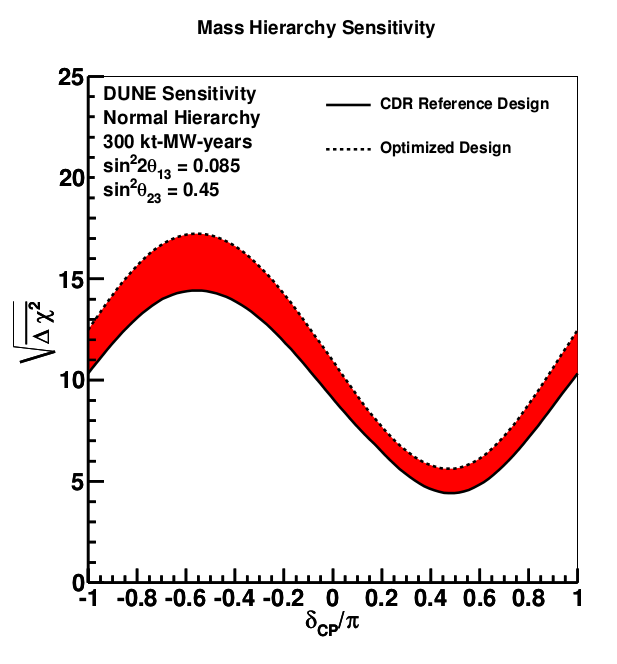
\includegraphics[width=0.30\textwidth, keepaspectratio=true]{figs/sensitivity_MH.png}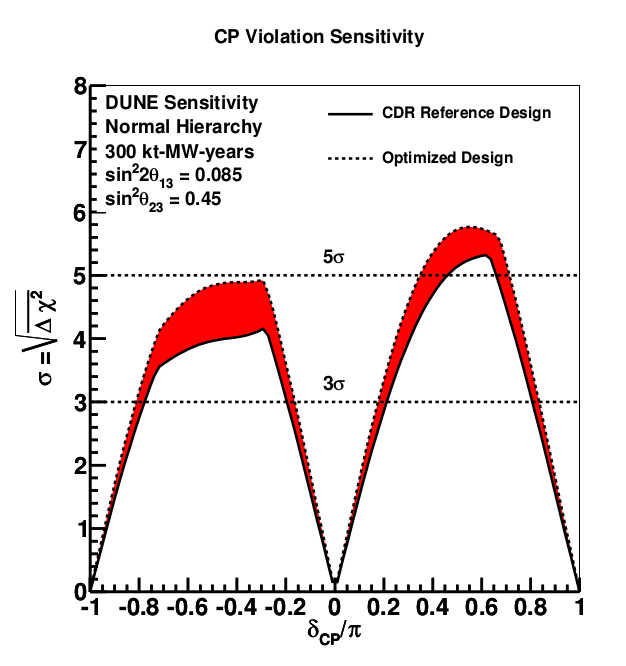
\includegraphics[width=0.31\textwidth, keepaspectratio=true]{figs/sensitivity_CP.png}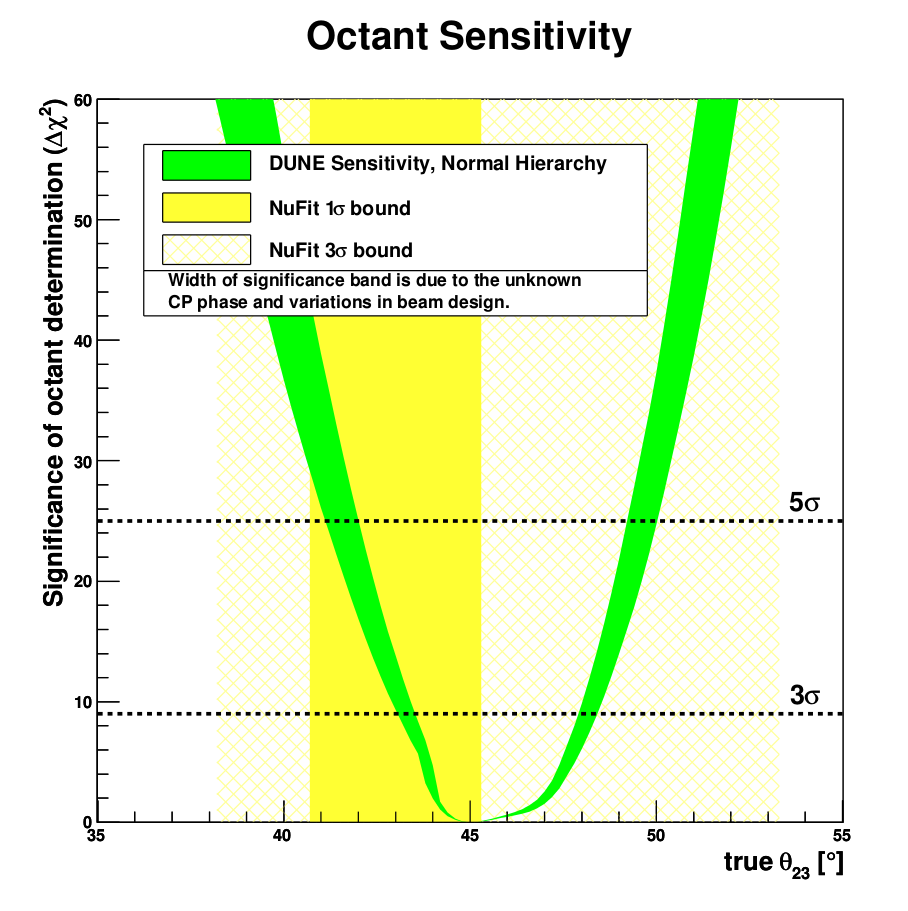
\includegraphics[width=0.32\textwidth, keepaspectratio=true]{figs/sensitivity_theta23.png}
\end{figure}
%%%%%%%%%%%%%%%%%%%%%%%%%%%%%%%%%%%%%%%%
%% if reference beam only
%%%%%%%%%%%%%%%%%%%%%%%%%%%%%%%%%%%%%%%%
%% if also has optimized beam
%\begin{table}[h]
%  \centering
%  \begin{center}
%  \caption{ The exposure needed to perform measurements with certain precision expressed in $MW \cdot kt \cdot years$. Estimates provided in the table assume normal mass hierarchy and best fit values of the known parameters }
%  \begin{tabular}{|c|c|c|}
%  \hline  
%  Physics milestone & Exposure, $MW \cdot kt \cdot years$ & Exposure, $MW \cdot kt \cdot years$ \\ \hline
%   & (reference beam) & (optimized beam) \\ \hline
%  $1^0$ $\theta_{23}$ resolution ($\theta_{23}~=~42^0$) & 70 & 45 \\ \hline
%  CPV at $3\sigma$ $(\delta_{CP}=+\pi/2)$ & 70 & 70 \\ \hline
%  CPV at $3\sigma$ $(\delta_{CP}=-\pi/2)$ & 160 & 100 \\ \hline
%  CPV at $5\sigma$ $(\delta_{CP}=+\pi/2)$ & 280 & 210 \\ \hline
%  MH at $5\sigma$ (at worst) & 400 & 230 \\ \hline
%  $10^0~\delta_{CP}$ resolution at $\delta_{CP}=0$ & 450 & 290 \\ \hline
%  CPV at $5\sigma$ $(\delta_{CP}=-\pi/2)$ & 525 & 320 \\ \hline
%  CPV at $5\sigma$, $50\%$ of $\delta_{CP}$ & 810 & 550 \\ \hline
%  CPV at $3\sigma$, $75\%$ of $\delta_{CP}$ & 1320 & 850  \hline
%  \label{tab:exposures_needed}
%  \end{tabular}
%  \end{center}
%\end{table}

\subsection{Neutrino Beam}

\begin{figure}
\caption{The neutrino beam production at the LBNF. Source of figure: \cite{ref_LBNFweb}}
\label{fig:LBNF_nuBeam}
\centering
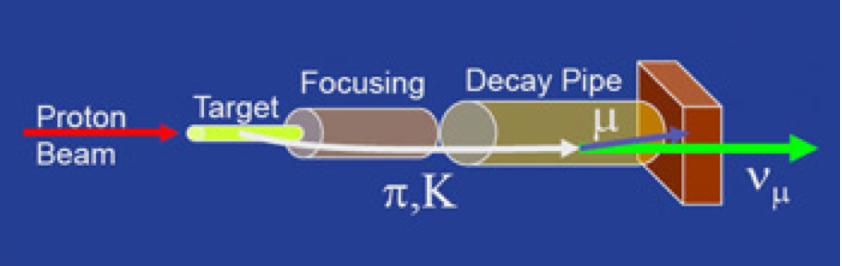
\includegraphics[width=0.45\textwidth, keepaspectratio=true]{figs/LBNF_nuBeam.png}  
\end{figure}


The LBNF neutrino beam will be the highest intensity neutrino beam ever created. The proton accelerator at Fermilab which was already used in other experiments at Fermilab before will produce the beam of protons. Then protons will hit a target and create pions through the reactions $p+p \rightarrow p+n+\pi^+$, $p+p \rightarrow p+\Delta^{++}+\pi^-$, $p+n \rightarrow p+p+\pi^-$, $p+n \rightarrow n+n+\pi^+$, $p+n \rightarrow p+\Delta^{-}+\pi^+$ and kaons through similar reactions which go strongly through gluon. 

%%%%%%%%%%%%%%%%%%%%%%%%%%%%%%%%%%%%%%%%%%%%%%%%%%%%%%
%% Feynman diagrams and descriptions of 
%% how the neutrinos were produced in the target 
%% are probably not necessary 
%%%%%%%%%%%%%%%%%%%%%%%%%%%%%%%%%%%%%%%%%%%%%%%%%%%%%%

%\begin{figure}
%\caption{Examples of the Feynmann diagrams of charged pion and kaon productions in proton-proton scattering.}
%\label{fig:pionAndKaonProductions}
%\centering
%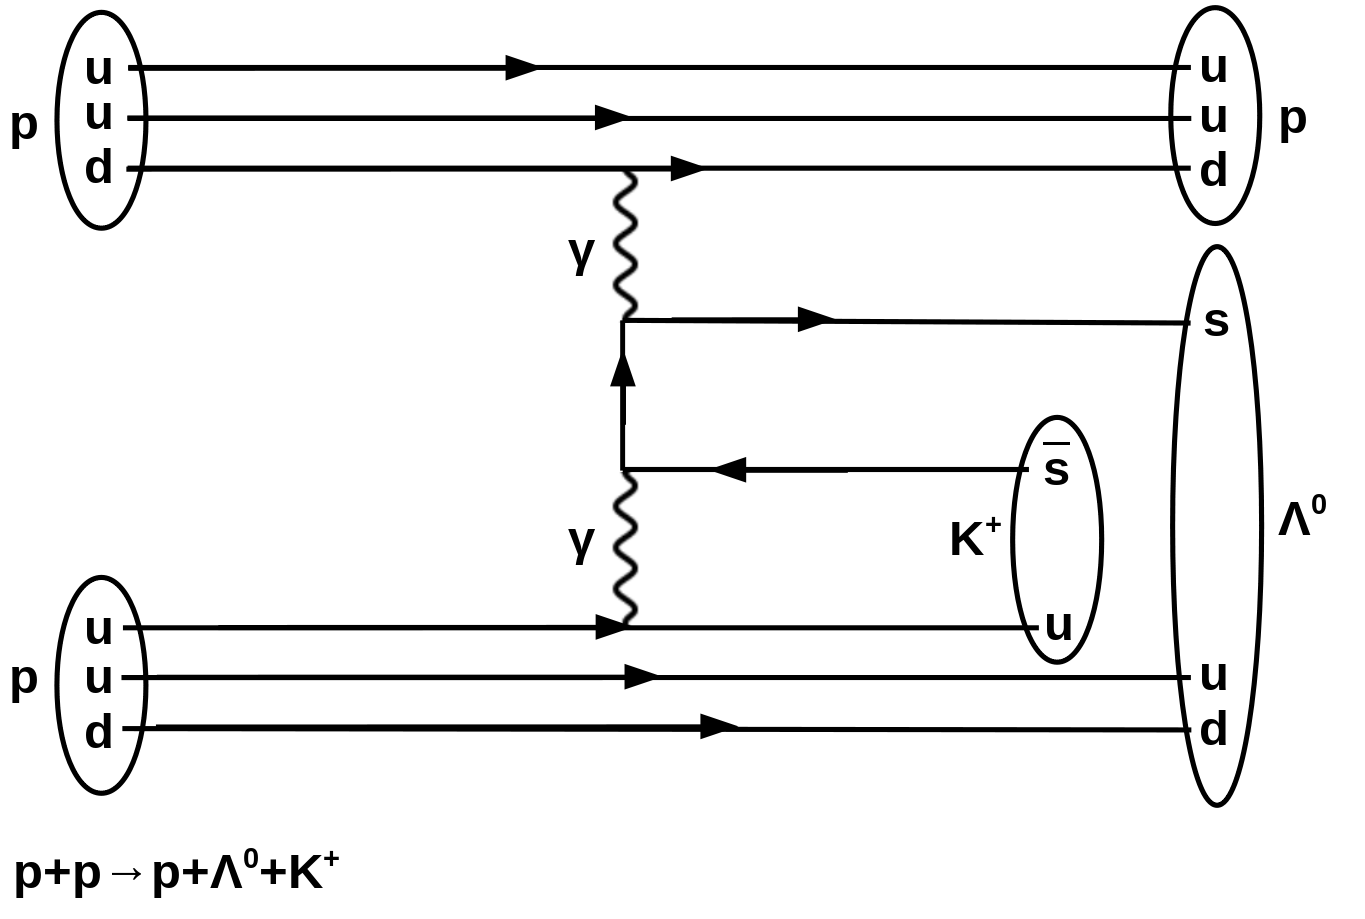
\includegraphics[width=0.48\textwidth, keepaspectratio=true]{figs/ppKaonProduction.png}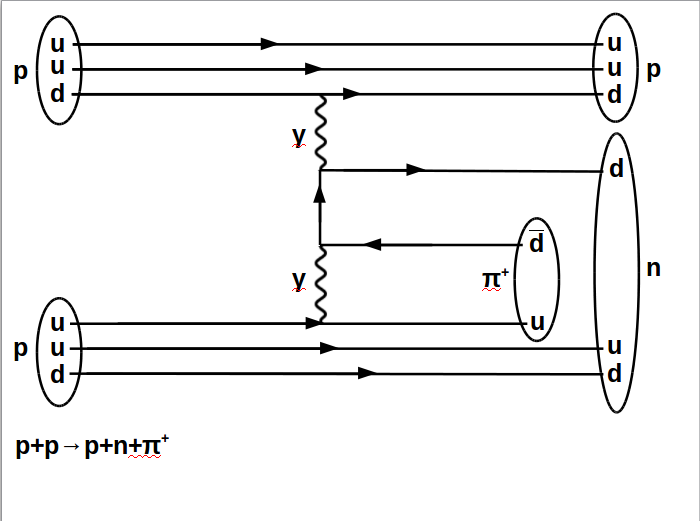
\includegraphics[width=0.48\textwidth, keepaspectratio=true]{figs/ppPionProduction.png}  
%\end{figure}
%In more general words, one quark from the accelerator beam proton scatters on the other quark from the proton or neutron of the target substance as shown at fig. \ref{fig:pionAndKaonProductions}. They exchange gluon which produces quark-antiquark pair. At this moment, the system has seven quarks and one antiquark. The antiquark pairs up with one of the quarks participating in the reaction and the remaining six quarks make two baryons in a way to satisfy color charge neutrality in final particles.  The charged pions have quark compositions $\pi^+ = u\bar{d}$ and $\pi^- = \bar{u}d$ and can be produced with the reactions which only include first generation quarks. The formulas of charged kaons are $K^+ = u\bar{s}$, $K^- = \bar{u}s$. Thus, to produce kaons, the gluon has to produce $s\bar{s}$ pair. 
%\begin{figure}
%\caption{Feynmann diagrams of charged pion and kaon decays to muon and muon antineutrino weakly through W-boson}
%\label{fig:pionAndKaonDecays}
%\centering
%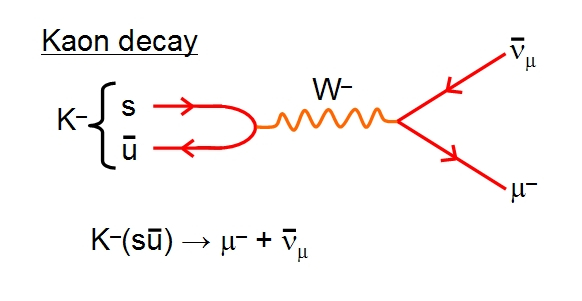
\includegraphics[width=0.45\textwidth, keepaspectratio=true]{figs/kaonDecay.jpg}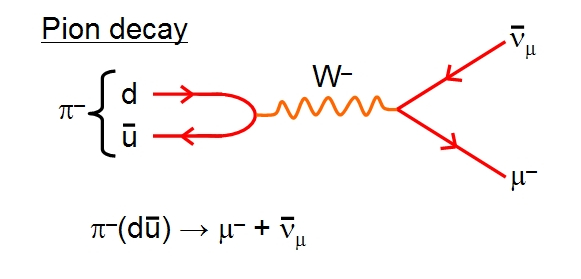
\includegraphics[width=0.45%\textwidth, keepaspectratio=true]{figs/pionDecay.jpg} 
%\end{figure}

After the mesons are created, they go through the focusing system and decay into the decay pipe as $\pi^+ \rightarrow \mu^+\nu_\mu$, $\pi^- \rightarrow \mu^-\bar{\nu_\mu}$, $K^+ \rightarrow \mu^+\nu_\mu$, $K^- \rightarrow \mu^-\bar{\nu_\mu}$ (fig. \ref{fig:pionAndKaonDecays}). The branching ratios of charged pions and kaons to decay into $\mu^+\nu_\mu$($\mu^-\bar{\nu_\mu}$) are $(>99.9)\%$ and $(63.55\pm0.011)\%$ respectively therefore most neutrinos produced into the decay pipe will be muon neutrinos. (While the neutral kaons can also be produced in the target and later decay in pions which could further decay and produce muon neutrinos, the focusing is being done with the certain configuration of the magnetic field and only can affect charged particles. Neutral pions, $\pi^0$s, are very likely to be produced as well but they decay as $\pi^0 \rightarrow \gamma\gamma$ and, therefore, can't contribute to the neutrino production.)\\
After being produced in the reactions described above, the neutrinos will be detected in the near detector at Fermilab. Then the neutrinos will travel 1300 km through the Earth crust and will be detected at SURF in South Dakota.\\  

One of the most important beam requirements is high intensity to produce large enough number of neutrinos to perform intended measurements. Expected beam power of 1.07 MW is expected in the beginning of the experiment with further update to 2.4 MW which is three times larger than the highest beam intensity from other experiments of this kind. Beam production system must be able to work in both muon neutrinos and muon antineutrinos modes. Energies of produced neutrinos must cover the first and the second oscillation nodes which corresponds to energies of 0.5-5 GeV for baseline of 1300 km. Corresponding proton energies are 60-120 GeV.


\subsection{Far Detector}

The main physics goal of the FD would be to measure $N_{\nu_e}(E_{\nu})$  from Formula \ref{eq:NnueEspectrum} but it would also measure $N_{\nu_\mu}(E_{\nu})$ to observe the reduced muon neutrino spectrum. Neutrinos and antineutrinos can produce signal through the CC:

$\nu_f+N \rightarrow f^- + N' +X$, $\bar{\nu_f}+N \rightarrow f^+ + N' +X$,

or through the NC:

$\nu_f+N \rightarrow \nu_f + N +X$, $\bar{\nu_f}+N \rightarrow \bar{\nu_f} + N +X$

where f is e or $\mu$, N is a proton or a neutron, N' is another baryon, and X is other hadrons produced in the reaction.

In case of CC, the produced charged lepton would be fully reconstructed, and also energy of all the final state particles would be summed up to reconstruct the neutrino energy. In case of NC, neutrino would not be detected, such events would be treated as a background.

The FD would be capable to efficiently reconstruct photons, electrons, muons and hadrons. \\

\begin{figure}
\caption{The scheme of the cross section of the LArTPC for far detector of the DUNE and the FD caverns. Sources of figures: \cite{ref_LBNF_CDR}}
\label{fig:farDetector_TPC}
\centering
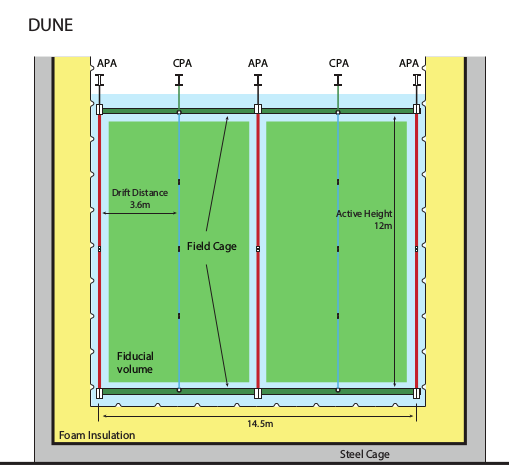
\includegraphics[width=0.5\textwidth, keepaspectratio=true]{figs/farDetector_TPC.png}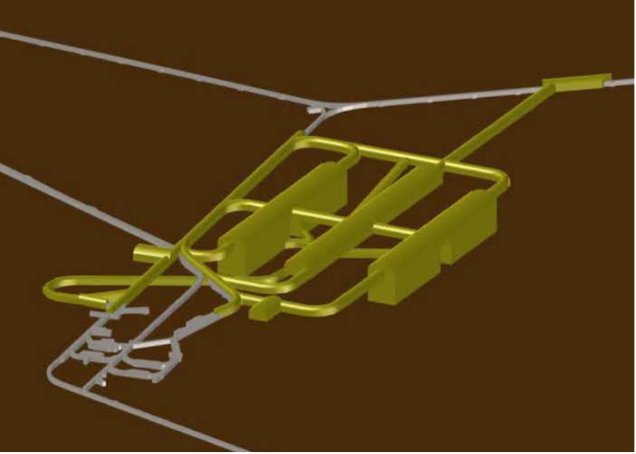
\includegraphics[width=0.5\textwidth, keepaspectratio=true]{figs/farDetector_Caverns.png}
\end{figure}

The LBNF/DUNE FD will be located at SURF in South Dakota. There will be four modules, 10,000 tonnes of liquid argon each, placed into four caverns 1500 m underground. Each module will be 15 m wide, 12 m high and 58 m long, along the beam direction. The caverns will be placed as pairs and there will be the fifth cavern between two pairs - the one with the cryogenic equipment, to provide cooling for liquid argon.\\ 

Key advantages of liquid argon as an FD working volume as described in \cite{ref_aboutLAr} are the ability to act as both a target and a detector, and also to operate as a tracker and a Cherenkov detector at the same time. Liquid argon is denser than water, and therefore such detector would experience more neutrino induced reactions per unit volume than a water detector would. \\

The liquid argon TPC is the main working volume of the detector. The chamber is merged into the liquid argon at a temperature of 89 K. In Figure \ref{fig:farDetector_TPC}, the cathode plane assemblies (CPAs) and the anode plane assemblies (APAs) are shown. The voltages on the APAs and the CPAs are applied in such a way to create a uniform electric field between anode and cathode planes. Charged particle traveling through the electron field ionizes argon atoms. Electrons induced in the ionization process drift to the APAs and produce signal on the readout electronic elements.



\subsection{Near Detector}

The most important physics goal of the ND is to measure the produced muon neutrino flux $\frac{dN_{\nu_\mu}(E_{\nu})}{dS}$ as it would go to Formula \ref{eq:NnueEspectrum}. In the $\nu_\mu$ beam there is also $\nu_e$ contamination present which would be background to $\nu_e$ which would appear as a result of neutrino oscillations at the FD. This background has to be estimated and subtracted. There would be also admixtures of $\bar{\nu_\mu}$ and $\bar{\nu_e}$ in the beam produced. The ND would perform measurement of the overall neutrino and antineutrino flavor composition. 

To measure flavor composition, the ND has to be able to reconstruct muons and electrons, and also to be able to distinguish between the opposite sign leptons. 

\begin{figure}
\caption{Scheme of the DUNE Near Detector (left) and related complex (right).}
\label{fig:nearDetector}
\centering
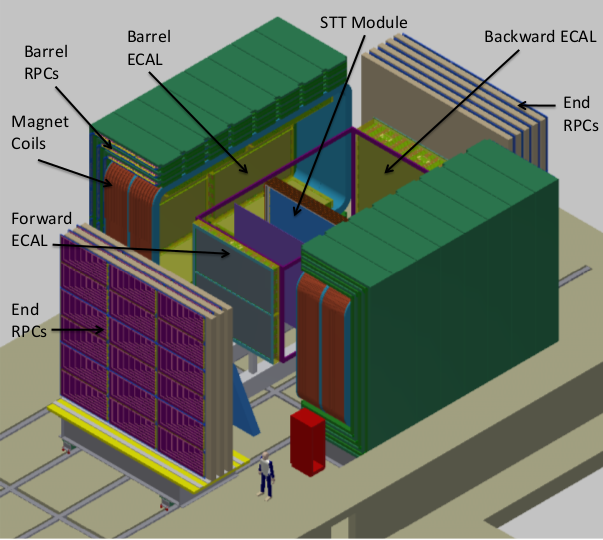
\includegraphics[width=0.63\textwidth, keepaspectratio=true]{figs/nearDetector.png}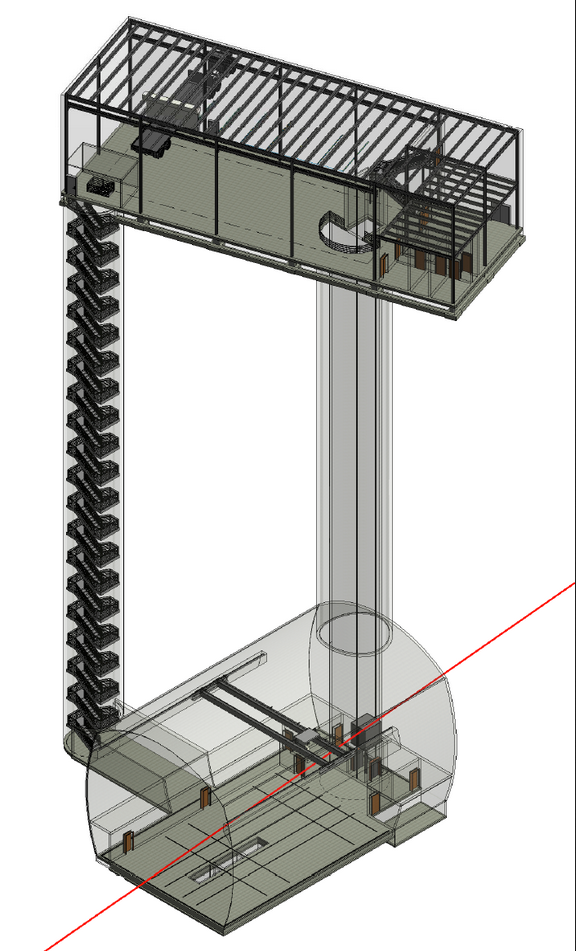
\includegraphics[width=0.35\textwidth, keepaspectratio=true]{figs/nearDetector_project.png}
\end{figure}

The ND would be located few hundred meters downstream the neutrino beam, and the neutrino beam would be much denser at this point than after travelling 1300 km to the FD, that is why the ND doesn't have to be as large as the FD. Also the ND aims on measuring number of neutrinos with much higher precision than the FD to significantly reduce the systematic uncerntainties.\\  

Because of different physics goals, the scheme of the ND (shown at the Fig. \ref{fig:nearDetector}) is also very different from the one of the FD. The detector will consist of central Straw-Tube Tracker (STT) modules, electromagnetic calorimeter (ECAL), magnet coils of 0.4T and muon identification system consisting of Resistive Plate Chamber (RPC) modules. The neutrinos would come from the bottom left corner of the picture, to the End RPCs. The detector will be placed 60 meters underground.





%\subsection{LBNF compared to the other long baseline neutrino oscillation experiments}
Table \ref{tab:compareExps} provides the comparisons of the LBNF/DUNE most important parameters with those of the other long baseline neutrino experiments: K2K, NuMI, CNGS and T2K \cite{ref_LBN_OscExpReview}. The beam power of LBNF/DUNE is planned to be 2.4 MW while the other operating experiments have only beam powers of few hundred Watts. The baseline of LBNF/DUNE is planned to be 1300 km while the baselines of the other experiments vary from 250 km to 735 km only. The Super-Kamiokande FD has a larger mass than the LBNF/DUNE FD is going to have (50 kt vs 40 kt) but the LBNF/DUNE FD will be filled with liquid argon which is a more favorable substance for neutrino detection than water (which the Super-Kamiokande FD is filled with). The only FD which has liquid argon as working volume is ICARUS but its mass is only 0.76 kt. \\ \\
%Therefore, among the experiments discussed, LBNF/DUNE is going to have the longest baseline, the highest beam power and the FD with the highest neutrino detection efficiency. These characteristics will allow LBNF/DUNE to perform more precise measurements than previous and currently existing experiments can do and become sensitive to effects which were not observed before.
\begin{table}[h]
  \centering
  \begin{center}
  \caption{ Comparison of different long baseline neutrino oscillations experiments. Abbreviations and notations used in the table: $E_p$ - proton energy, FGD - Fine-Grained Detector, ChD - Cherenkov Detector, LAr - liquid argon }
  \begin{tabular}{|c|c|c|c|c|c|}
              & KEK (K2K) & NuMI & CNGS & T2K & LBNF/DUNE\\ \hline
     location & Japan  & Illinois - & Switzerland - & Japan & Illinois - \\ 
              &        & Minnesota & Italy &  & South Dakota\\ \hline
     accelerator & KEK PS  & FNAL & CERN's SPS & J-PARC & FNAL\\ \hline
     time of oper. & 1999-2004  & 2005-2012 & 2006-2012 & 2010- & future \\ \hline 
     beam power  &  5 kW  & 300-350 kW  & 300 kW & 750 kW & 2400 kW\\ \hline 
     $E_p$  & 12 GeV & 120 GeV & 400 GeV & 30 GeV & 60-120 GeV\\ \hline 
     baseline  & 250 km & 735 km & 730 km & 295 km & 1300 km\\ \hline 
%                & KEK (K2K)   & NuMI                & CNGS                & T2K         & LBNF (DUNE)\\ \hline
     near        & (water ChD) & MINOS               & (muon               & ND280       & DUNE (FGD)\\  
     detector(s) & (FGD)       & (track. and scint.) & detector)           & INGRID      & \\ \hline 
     ND mass     & 1 kt (ChD)  & 0.98 kt             &                     &             & \\ \hline 
     far         & SuperK      & MINOS               & ICARUS (LAr)        & SuperK      & DUNE (LAr)\\  
     detector(s) & (water ChD) & track. and scint.   & OPERA (FGD)        & (water ChD) & \\ \hline 
     FD mass     & 50 kt       & 5.4 kt              & 0.76 kt (ICARUS)   & 50 kt       & 40 kt\\ 
                 &             &                     & 1.25 kt (OPERA)    &             & \\ \hline 
 \end{tabular}
  \label{tab:compareExps}
  \end{center}
\end{table}

% Summary
LBNF/DUNE is future long baseline neutrino oscillations experiment which will be hosted by two large physics laboratories in USA: Fermilab in Illinois and SURF in South Dakota. LBNF/DUNE's baseline of 1300 km, expected beam power of 2 MW, and 40 kt of liquid argon FD makes LBNF/DUNE the most ambitious neutrino oscillations facility ever created. In addition to precision measurements of neutrino mixing parameters such as $\theta_{12}$, $\theta_{23}$, $\theta_{13}$, $|\Delta{m_{12}}^2|$, $|\Delta{m_{32}}^2|$, it is expected to have enough sensitivity to determine the neutrino mass hierarchy and the CP-violation phase $\delta$ which have never been previously determined.\\ \\
